\documentclass[11pt]{article}
\usepackage{geometry,marginnote} % Pour passer au format A4
\geometry{hmargin=1cm, vmargin=1cm} % 

% Page et encodage
\usepackage[T1]{fontenc} % Use 8-bit encoding that has 256 glyphs
\usepackage[english,french]{babel} % Français et anglais
\usepackage[utf8]{inputenc} 

\usepackage{lmodern,numprint}
\setlength\parindent{0pt}

% Graphiques
\usepackage{graphicx,float,grffile,units}
\usepackage{tikz,pst-eucl,pst-plot,pstricks,pst-node,pstricks-add,pst-fun,pgfplots} 

% Maths et divers
\usepackage{amsmath,amsfonts,amssymb,amsthm,verbatim}
\usepackage{multicol,enumitem,url,eurosym,gensymb,tabularx}

\DeclareUnicodeCharacter{20AC}{\euro}



% Sections
\usepackage{sectsty} % Allows customizing section commands
\allsectionsfont{\centering \normalfont\scshape}

% Tête et pied de page
\usepackage{fancyhdr} \pagestyle{fancyplain} \fancyhead{} \fancyfoot{}

\renewcommand{\headrulewidth}{0pt} % Remove header underlines
\renewcommand{\footrulewidth}{0pt} % Remove footer underlines

\newcommand{\horrule}[1]{\rule{\linewidth}{#1}} % Create horizontal rule command with 1 argument of height

\newcommand{\Pointilles}[1][3]{%
  \multido{}{#1}{\makebox[\linewidth]{\dotfill}\\[\parskip]
}}

\newtheorem{Definition}{Définition}

\usepackage{siunitx}
\sisetup{
    detect-all,
    output-decimal-marker={,},
    group-minimum-digits = 3,
    group-separator={~},
    number-unit-separator={~},
    inter-unit-product={~}
}

\setlength{\columnseprule}{1pt}

\begin{document}

\textbf{Nom, Prénom :} \hspace{8cm} \textbf{Classe :} \hspace{3cm} \textbf{Date :}\\

\vspace{-0.5cm} \begin{center}
  \textit{L'intelligence est insipide sans altruisme.}  - \textbf{Michel Bouthot}
\end{center}

\textbf{Théorème de Pythagore : } \dotfill \\
\Pointilles[1]

\subsubsection*{Ex1 : Pythagore rapide}
\textbf{Écrire le calcul et le résultat.}
  
\begin{figure}[H]
  \centering
  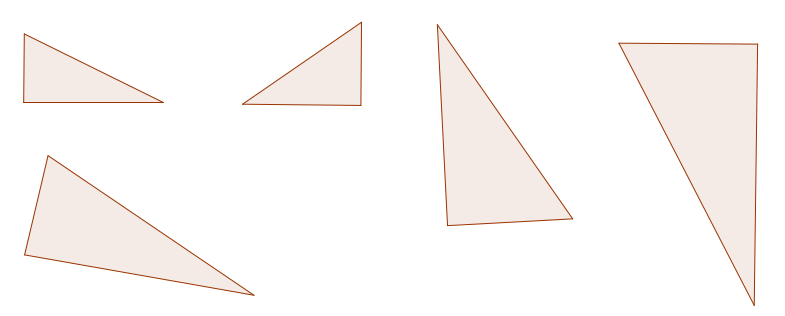
\includegraphics[width=0.6\linewidth]{4x8-pythagore-2/ex2.png}
\end{figure}

  \begin{enumerate}
  \item[a.] \dotfill 
  \item[b.] \dotfill 
  \item[c.] \dotfill 
  \item[d.] \dotfill 
  \item[e.] \dotfill 
  \end{enumerate}


\begin{multicols}{2}

  \subsubsection*{Ex2 : Pythagore Rédaction}

  Soit RTL un triangle rectangle en R tel que : RT = 37,5 cm et TL = 48,5 cm. \\
  \textbf{Calculer la longueur RL.}

  \Pointilles[16] \columnbreak

  \subsubsection*{Ex3 : Pythagore Réciproque}

  Soit RTL un triangle tel que : RT = 15,5 cm, RL = 25,5cm et TL = 20,5 cm. \\
  \textbf{Le triangle est-il rectangle ?}

\Pointilles[16]

\end{multicols}

\newpage

\subsubsection*{pb1. Second poteau Pavard} 

\begin{multicols}{2}

Lors du match de foot France - Argentine du 30 Juin 2018, Pavard (P) met une sublime reprise de volée sur une passe décisive de Lucas (L). La balle terminant dans le but adverse (B).

\url{https://www.youtube.com/watch?v=9nECmaDC5A4}

Pour analyse de l'action, on récupère des données. 

\begin{itemize}
  \item Distance entre Pavard et Lucas : PL = 45m
  \item Distance entre Pavard et le But : PB = 22m
  \item Distance entre le But et Lucas : BL = 40m
\end{itemize}

\textbf{Le triangle formé par Pavard, Lucas et le But est-il rectangle ?} \columnbreak

\begin{figure}[H]
  \centering
  \includegraphics[width=\linewidth]{4x8-pythagore-2/pb1.pdf}
\end{figure}

\end{multicols}

\Pointilles[10]

\begin{multicols}{2}

\subsubsection*{pb2. The Wind Waker} 

Dans The Wind Waker, Link doit réparer la voile triangulaire de son bateau. Pour cela, il doit coudre un fils le long des trois côtés du triangle. 

\textbf{Calculer le périmètre du triangle formé par la voile.} 

\Pointilles[9] \columnbreak

\begin{figure}[H]
  \centering
  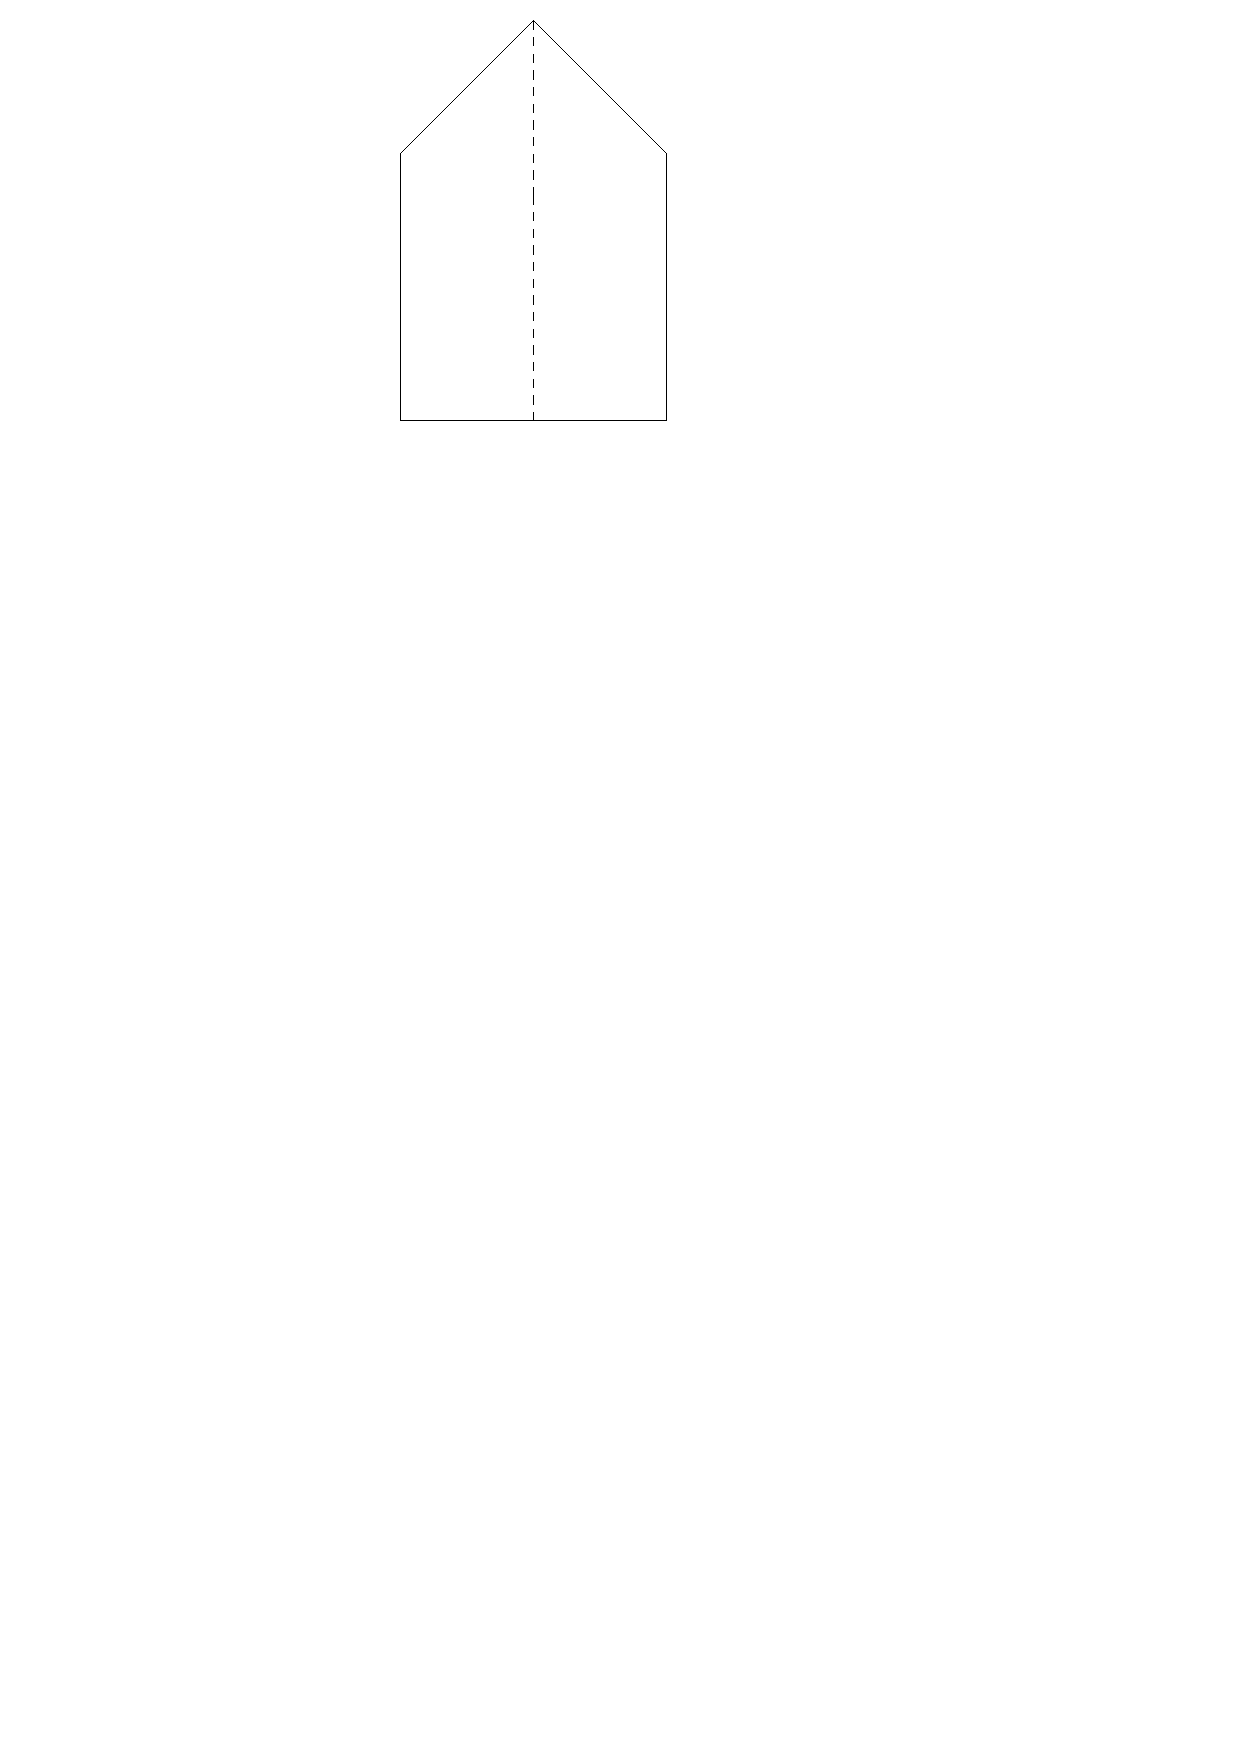
\includegraphics[width=0.8\linewidth]{4x8-pythagore-2/pb2.pdf}
\end{figure}

\end{multicols}

\Pointilles[7]

\end{document}